%----------------------------------------------------------------------------------
% Exemplo do uso da classe tcc.cls. Veja o arquivo .cls
% para mais detalhes e instruções.
%----------------------------------------------------------------------------------
\chapter{Fundamentação Teórica}\label{chap2:fund_teo}
    \section{USV}\label{subchap2:USV}
        \textit{"Unmanned Surface Vehicle"}, ou veículo de superfície não tripulado, é caracterizado por realizar atividades navais de forma autônoma, ou controlado remotamente, sem a presença de tripulação.~\cite{LIU201671} Tais caracteríscticas também enquadram um USV na categoria de um robô.~\cite{JURAK2020}
        
        De acordo com Liu~\cite{LIU201671}, um USV pode ter as mais variadas aparências e funcionalidades, porém os seguintes componentes básicos devem compor um USV:
        
        \begin{enumerate}
            \item Casco e estruturas mecânicas auxiliares
            \item Sistema de Propulsão
            \item Sistema GNC (\textit{"Guidance Navigation and Control"})
            \item Sistema de Comunicação
            \item Equipamento de Coleta de Dados
            \item Estação de Solo
        \end{enumerate}
        
        Dentre os elementos listados o sistema GNC é fundamental para automatizar um USV, pois ele controlará o sistema do USV como um todo. Sua função consiste coletar informações a respeito do USV e seu entorno (\textit{"Navigation"}), determinar o melhor caminho a seguir com base nos dados coletados (\textit{"Guidance"}) e executar as ações necessárias para seguir a melhor rota encontrada (\textit{"Control"}).  ~\cite{LIU201671} ~\cite{JURAK2020}
        
        \begin{figure}
            \centering
            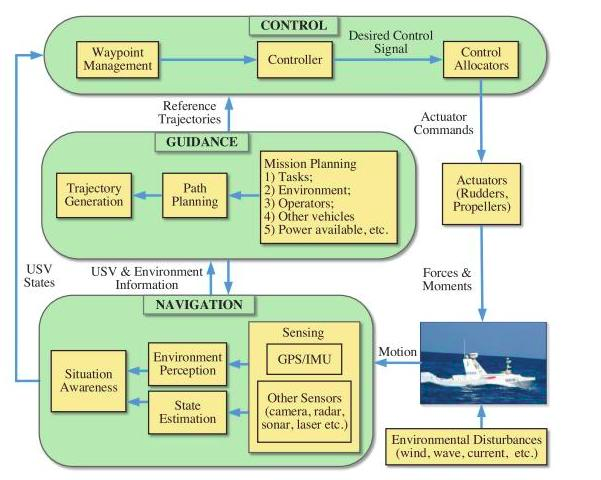
\includegraphics[width=\textwidth]{fig/gnc_system.png}
            \caption{Caption}
            \label{fig:gnc_system}
        \end{figure}
    
        A Figura ~\ref{fig:gnc_system} apresentada por Liu ~\cite{LIU201671} mostra o sistema GNC em detalhe apontando suas funções. Tais funções serão brevemente explicadas a seguir.
        
        \begin{enumerate}
            \item [1] \textit{"Navigation":} subsistema responsável pela coleta de informações a respeito do barco (posição, velocidade, etc) e seu entorno (obstáculos estáticos e obstáculos móveis). Essas informações são coletadas por meio de sensores, radares, câmeras, cartas náuticas e mapas. Os dados coletados são enviados para o subsistema \textit{"Guidance"}.~\cite{JURAK2020}
            
            \item [2] \textit{"Guidance":} subsistema reponsável por analisar os dados recebidos do subsistema \textit{"Navigation"} e encontrar o melhor trajeto possível, através de planejadores, para atingir o objetivo.~\cite{JURAK2020} Portanto, é responsabilidade do subsistema \textit{"Guidance"} executar todas as etapas necessárias para a prevenção de colisão~\cite{HUANG2020451}, que serão abordadas na sessão ~\ref{subchap2:prev_col}.
            
            \item [3] \textit{"Control":} subsistema que origina os comandos necessários para seguir a rota traçada pelo subsistema \textit{"Guidance"}. Além disso, também é sua responsabilidade executar os comandos gerados diretamente nos atuadores do USV.~\cite{JURAK2020}
        \end{enumerate}
    
    \section{COLREGS}\label{subchap2:colregs}
        Buscando padronizar as ações tomadas para evitar colisões a Organização Internacional da Marinha (IMO - do inglês International Marine Organization) definiu uma série de regulamentações para colisão no mar (COLREGS - do inglês COLlision REGulations at Sea).~\cite{JURAK2020}
        
        Para que o uso de USV não apresente perigo para outras embarcações triupuladas, é necessário que ele não realize ações inesperadas pelos humanos do barco que se aproxima. Sendo assim, o USV deverá realizar suas ações de acordo com a COLREGS de forma que seja perceptível para o humano que estiver no outro barco.~\cite{KUWATA2014110}
        
        Jurak~\cite{JURAK2020} em seu sistema considerou os seguintes encontros: 
        
        \begin{enumerate}
            \item [1] \textit{"head-on":}
            \item [2] \textit{"crossing from left"}
            \item [3] \textit{"crossing from right"}
            \item [4] \textit{"overtaking"}
        \end{enumerate}
        
        
        
    
    \section{Prevenção de Colisão}\label{subchap2:prev_col}
        Uma tarefa primordial quando se trata de navegação é evitar que a embarcação colida com algum obstáculo. Porém, é alto o número de acidentes com embarcações envolvendo colisões. Além disso, diversas investigações apontam que a principal causa desses acidentes é o fator humano.~\cite{HUANG2020451}
        
        Frente ao alto número de ocorrencias dessa natureza, pesquisadores vem estudando meios de evitar tais acidentes. [Huang] afirma que atualmente há duas frentes na tecnologia de prevenção de colisão: (1) assitência à tripulação e (2) eliminação de fatores humanos. Sendo esta última a perspectiva abordada neste trabalho dado que o componente físico de implementação é um USV.~\cite{HUANG2020451}
        
        Huang (2020, p.2) define prevenção de colisão como:
        \begin{directcite}
            \textit{"Prevenção de colisão é o processo em que um navio desvia de sua trajetória planejada para evitar contato físico indesejado em um certo tempo futuro"}
        \end{directcite}
        
        Com isso, [Huang] separa o processo de prevenção de colisão nas etapas de "detecção de conflito", que determina se o navio está em risco de colisão ou não, e "resolução de conflito", que define quais ações devem ser tomadas pelo navio para evitar a colisão. Em um USV, tais atividades são atribuidas ao módulo de \textit{"Guidance"} do sistema GNC.~\cite{HUANG2020451}
        
        Na Figura~\ref{fig:col_avoid_info_flow} é possível observar o fluxo de informação por entre os módulos que compõe um sistema de evasão de colisão. Em suma, o módulo \textit{"Observer"} coleta informações através de seus sensores e câmeras; \textit{"Motion Prediction"} faz uso dos dados coletados pelo módulo anterior para estimar as futuras posições do OS e do TS; \textit{"Conflict Detection"} ineterpreta as informações fornecidas pelos módulos anteriores para verificar se há o risco de colisão; havendo risco de colisão, o módulo \textit{"Conflict Resolution"} é acionado para determinar as ações necessárias para evadir da situação de risco; o módulo \textit{"Actuator"} executa as ações definidas pelos módulos anteriores.~\cite{HUANG2020451}
        
        \begin{figure}
            \centering
            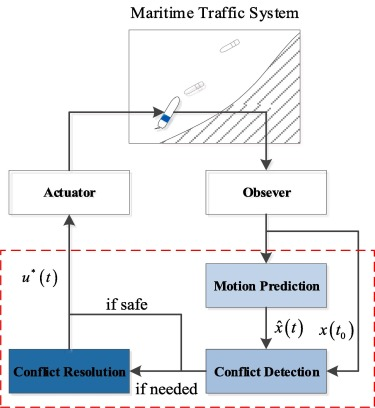
\includegraphics{fig/information_flow.png}
            \caption{Fluxo de informação ~\cite{HUANG2020451}}
            \label{fig:col_avoid_info_flow}
        \end{figure}
        
        Os módulos envoltos ao pontilhado vermelho na Figura~\ref{fig:col_avoid_info_flow} formam o sistema de evasão de colisão. 